\documentclass[../ZF_Wing.tex]{subfiles}
\begin{document}

\textcolor {pink} {Hauptaufgaben Kalkulation}
\begin{enumerate}
	\item Ermittlung Selbstkosten (Total-Kosten)
	\item Die Preisfindung
	\item Die Preisbeurteilung
	\item Die Offertenerstellung
\end{enumerate}


\subsection{Kalkulation im Industriebetrieb}

Mit Gemeinskonstenzuschlagsätzen: Korrekter Preis bestimmen in der Einzelkalkulation
\paragraph{Kalkulation Schema 1\\}
\textbf{Materialkosten =} Einzel-Material + Material-Gemeinkosten\\
\\
\textbf{Fertigungskosten =} Einzel-Löhne + Fertigungs-Gemeinkosten\\
\\
\textbf{Herstellkosten =} Materialkosten + Fertigungskosten\\
\\
\textbf{Selbstkosten =} Herstellkosten + Verwaltungs-Gemeinkosten\\
\\
\textbf{Nettoerlös(Netto-Verk.Preis exkl.MwSt.!!!)=} Selbstkosten + Reingewinn


\paragraph{Kalkulation Schema 2\\}


\textbf{Nettobarverkaufspreis =} Nettoverkaufspreis + Verkaufssonderkosten\\
\\
\textbf{Nettokreditverkaufspreis =} Nettobarverkaufspreis + Skonto\\
\\
\textbf{Bruttokreditverkaufspreis =} Nettokreditverkaufspreis + Rabatt\\
\\
\textbf{Bruttokreditverkaufspreis inkl. MwSt. =} Bruttokreditverkaufspreis + MwSt

\paragraph{Kalkulation:\\}
1. Zuschlagsätze ermitteln\\
\\
2. Schema 1 oder Schema 2 verwenden\\
\\

\subsection{Kalkulation Handelsbetrieb}

\textbf{Besteht aus 3 Teilen:}
\begin{itemize}
	\item Einkaufs-Kalkulation
	\item Betriebs-Kalkulation
	\item Verkaufs-Kalkulation
\end{itemize}


\paragraph{\colorbox{orange!30}{Einkaufskalkulation Schema:}\\}

\textbf{Nettokreditankaufspreis(=Rechnungsbetrag)=} Bruttokreditankaufspreis(= Katalogpreis des Lieferanten) - Rabatt\\
\\
\textbf{Nettobareinkaufspreis =} Nettokreditankaufspreis - Skonto\\
\\
\textbf{Einstandswert/Einstandspreis =} Nettobareinkaufspreis + Bezugskosten\\
\\


\paragraph{\colorbox{orange!30}{Betriebsinterne-Kalkulation Schema:}\\}

\textbf{Selbstkosten = } Einstandswert + Gemeinkosten\\
\\
\textbf{Nettoverkaufspreis (Nettoerlös)=} Selbstkosten + Reingewinn\\
\\

\paragraph{\colorbox{orange!30}{Verkaufs-Kalkulation Schema}\\}


\textbf{Nettobarverkaufspreis =} Nettoverkaufspreis + Verkaufssonderkosten\\
\\
\textbf{Nettokreditverkaufspreis =} Nettobarverkaufspreis + Skonto\\
\\
\textbf{Bruttokreditverkaufspreis =} Nettokreditverkaufspreis + Rabatt\\

\paragraph{\colorbox{orange!30}{Verkaufs-Kalkulation Gesamt-Kalkulation}\\}

Vom Katalogpreis zum eigenen Katalog-/Ladenpreis\\

\begin{figure}[H]
\centering
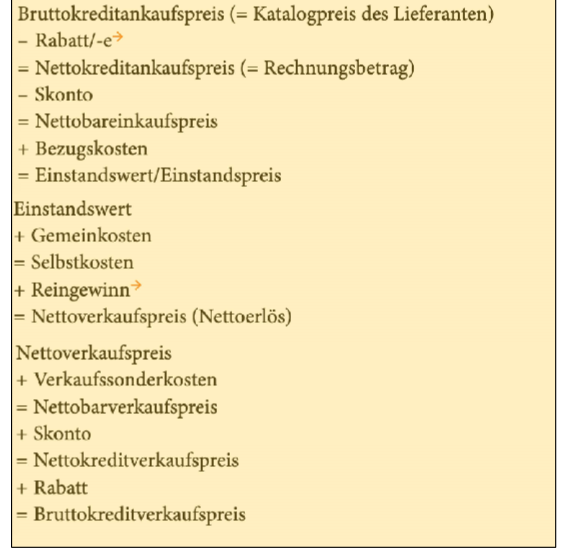
\includegraphics[width=0.3\textwidth]{Resources/Image/Gesamt-Kalkulation.png}
\caption{\label{fig:Gesamt-Kalkulation}Gesamt-Kalkulation.}
\end{figure}

























































































































































































\end{document}